\section{Results and Analysis}\label{results-and-analysis}

\subsection{Split-Aware Mainline and Reference Summary}\label{split-aware-mainline-and-reference-summary}

To avoid cross-split misreading, the thesis now separates the segmentation mainline table (\texttt{val71}) from the locked reference table (\texttt{test73}).

\textbf{Table 5.1: T28 mainline on \texttt{val71} (primary evidence tier)}

{\def\LTcaptype{none} % do not increment counter
\begin{longtable}[]{@{}lcccl@{}}
\toprule\noalign{}
Route & Split & PQ@0.5 & BM-Dice & Note \\
\midrule\noalign{}
\endhead
\bottomrule\noalign{}
\endlastfoot
T28 (seed42) & \texttt{val71} & 0.686 & 0.819 & Single-seed best checkpoint \\
T28 (seed123) & \texttt{val71} & 0.681 & 0.815 & Single-seed best checkpoint \\
\textbf{T28 mainline (dual-seed mean)} & \textbf{\texttt{val71}} & \textbf{0.684} & \textbf{0.817} & \textbf{Sealed thesis mainline} \\
\end{longtable}
}

\textbf{Table 5.2: Locked baseline references on \texttt{test73} (context tier)}

{\def\LTcaptype{none} % do not increment counter
\begin{longtable}[]{@{}
  >{\raggedright\arraybackslash}p{(\linewidth - 10\tabcolsep) * \real{0.1860}}
  >{\centering\arraybackslash}p{(\linewidth - 10\tabcolsep) * \real{0.1860}}
  >{\centering\arraybackslash}p{(\linewidth - 10\tabcolsep) * \real{0.2093}}
  >{\centering\arraybackslash}p{(\linewidth - 10\tabcolsep) * \real{0.1163}}
  >{\centering\arraybackslash}p{(\linewidth - 10\tabcolsep) * \real{0.1628}}
  >{\raggedright\arraybackslash}p{(\linewidth - 10\tabcolsep) * \real{0.1395}}@{}}
\toprule\noalign{}
\begin{minipage}[b]{\linewidth}\raggedright
Method
\end{minipage} & \begin{minipage}[b]{\linewidth}\centering
PQ@0.5
\end{minipage} & \begin{minipage}[b]{\linewidth}\centering
BM-Dice
\end{minipage} & \begin{minipage}[b]{\linewidth}\centering
AJI
\end{minipage} & \begin{minipage}[b]{\linewidth}\centering
F1
\end{minipage} & \begin{minipage}[b]{\linewidth}\raggedright
Note
\end{minipage} \\
\midrule\noalign{}
\endhead
\bottomrule\noalign{}
\endlastfoot
Cellpose v4.0.1 (\texttt{d=250}) & 0.120 & 0.362 & 0.189 & 0.182 & \texttt{test73}, single-checkpoint locked reference \\
SAM ViT-B & 0.286 & 0.631 & 0.440 & 0.492 & \texttt{test73}, single-checkpoint locked reference \\
CellSAM (pretrained) & 0.434 & 0.682 & 0.499 & 0.636 & \texttt{test73}, single-checkpoint locked reference \\
MedSAM & 0.576 & 0.771 & 0.634 & 0.834 & \texttt{test73}, single-checkpoint locked reference \\
T27a Plan B Decoder-Only & 0.659 & 0.800 & 0.669 & 0.960 & \texttt{test73}, single-checkpoint historical reference \\
\end{longtable}
}

\textit{Aggregation note.} \texttt{F1} denotes split-level micro-\texttt{F1} computed from aggregated \texttt{TP/FP/FN} at IoU$=0.5$.

Three conclusions follow from Tables 5.1 and 5.2.

First, the primary segmentation claim is anchored to T28 dual-seed \texttt{val71} mean (\texttt{PQ\ =\ 0.684}, \texttt{BM-Dice\ =\ 0.817}), not to any single-checkpoint \texttt{test73} row.

Second, locked \texttt{test73} references remain necessary for baseline context and audit traceability. The latest-version Cellpose rerun stays weak (\texttt{PQ\ =\ 0.120}), while the audited CellSAM-family and MedSAM references preserve historical comparability. Detailed branch-level audit evidence, including the \texttt{model/model\_cp} divergence, is documented in Appendix~A (\S\ref{detailed-audit-of-the-released-cellsam-checkpoint}).

Third, split separation is intentional: \texttt{val71} mainline and \texttt{test73} references are not used for direct horizontal superiority claims.

For detector-driven integration, T28 remains the fixed segmentation backend. This selection is based on consistent multi-channel gains in the T28/T29 line and stronger detector-coupled end-to-end behavior in the latest detector-integration summaries.

\subsection{Loss Ablation}\label{loss-ablation}

The most reliable ablation evidence currently comes from T12, which was run with two seeds and evaluated on \texttt{test73}. These ablations are historically earlier than the current T28 mainline, but they remain useful because they explain why the current training recipe kept some design choices and removed others. The compared loss families are built from Dice \cite{milletari2016vnet}, AJI \cite{kumar2017aji}, Boundary \cite{kervadec2019boundary}, and Focal \cite{lin2017focal} components.

\textbf{Table 5.3: T12 loss ablation on \texttt{test73} (mean of 2 seeds)}

{\def\LTcaptype{none} % do not increment counter
\begin{longtable}[]{@{}lcccc@{}}
\toprule\noalign{}
Configuration & PQ & BM-Dice & AJI & dPQ \\
\midrule\noalign{}
\endhead
\bottomrule\noalign{}
\endlastfoot
Full (Phase 1, \texttt{posw\ =\ 2}) & 0.453 & 0.707 & 0.550 & - \\
BCE + Dice only & 0.459 & 0.711 & 0.554 & +0.6 \\
w/o BoundaryLoss & 0.454 & 0.708 & 0.554 & +0.1 \\
\textbf{w/o ContourLoss} & \textbf{0.476} & \textbf{0.718} & \textbf{0.564} & \textbf{+2.3} \\
w/o AJI loss & 0.459 & 0.710 & 0.554 & +0.6 \\
w/o PQ early stopping & 0.459 & 0.710 & 0.555 & +0.6 \\
\textbf{\texttt{pos\_weight\ =\ 10}} & \textbf{0.494} & \textbf{0.724} & \textbf{0.573} & \textbf{+4.1} \\
\end{longtable}
}

Two findings are robust enough to keep in the thesis body.

\begin{itemize}
\tightlist
\item
  \textbf{ContourLoss is harmful} on this dataset. Removing it gives a \texttt{+2.3} PQ gain, suggesting that the contour-driven penalty is too restrictive for elongated and irregular cardiomyocyte boundaries.
\item
  \textbf{\texttt{pos\_weight\ =\ 10} is critical}. This is the strongest single ablation gain and reflects the severe foreground-background imbalance inside box prompts.
\end{itemize}

These observations do not by themselves define the final T28 writing route, because T28 inherits the same combined-loss family while also changing channel handling. But they do explain why the historical Best Config moved away from the original Phase 1 setting, and why the thesis should not revert to the older \texttt{pos\_weight\ =\ 2} configuration when describing model evolution.

\subsection{Oracle-to-End-to-End Gap (Historical T27a Reference)}\label{oracle-to-end-to-end-gap-historical-t27a-reference}

The deployment bottleneck is currently the detection stage rather than the segmentation model itself. Table 5.4 reports the historical T27a reference comparison between Oracle prompting and automatically generated prompts on \texttt{test73}. The role of this table is diagnostic rather than mainline sealing.

\textbf{Table 5.4: Oracle vs end-to-end evaluation for historical T27a reference on \texttt{test73}}

{\def\LTcaptype{none} % do not increment counter
\begin{longtable}[]{@{}
  >{\raggedright\arraybackslash}p{(\linewidth - 8\tabcolsep) * \real{0.2581}}
  >{\centering\arraybackslash}p{(\linewidth - 8\tabcolsep) * \real{0.1290}}
  >{\centering\arraybackslash}p{(\linewidth - 8\tabcolsep) * \real{0.1290}}
  >{\centering\arraybackslash}p{(\linewidth - 8\tabcolsep) * \real{0.2903}}
  >{\raggedright\arraybackslash}p{(\linewidth - 8\tabcolsep) * \real{0.1935}}@{}}
\toprule\noalign{}
\begin{minipage}[b]{\linewidth}\raggedright
Setting
\end{minipage} & \begin{minipage}[b]{\linewidth}\centering
PQ
\end{minipage} & \begin{minipage}[b]{\linewidth}\centering
F1
\end{minipage} & \begin{minipage}[b]{\linewidth}\centering
BM-Dice
\end{minipage} & \begin{minipage}[b]{\linewidth}\raggedright
Note
\end{minipage} \\
\midrule\noalign{}
\endhead
\bottomrule\noalign{}
\endlastfoot
Oracle (GT boxes) & 0.659 & 0.960 & 0.800 & Reference main result \\
DAPI nuclear detection & 0.252 & 0.433 & 0.599 & \texttt{locked\_eval} \\
Adaptive Z-line detection & 0.293 & 0.497 & 0.612 & Better current E2E branch \\
\end{longtable}
}

Even with the better Adaptive Z-line detector, the gap from Oracle to end-to-end remains large: \texttt{-0.366} PQ and \texttt{-0.188} BM-Dice relative to Oracle. This means the segmentation model is already strong when the prompt is correct, but prompt quality remains the limiting factor for practical deployment.

This gap also explains why the thesis should keep Oracle and end-to-end results conceptually separate. Oracle tables answer whether the segmentation model itself works; end-to-end tables answer whether the whole pipeline is ready for use.

\subsection{T29 Channel Encoding and Adapter Decision}\label{t29-channel-encoding-and-adapter-decision}

T29 is retained in the main body as a focused channel-encoding ablation under dual-seed means. The objective is to isolate the contribution of adding DAPI and Actn2 cues under the official encoding family.

\textbf{Table 5.5: T29 channel-encoding ablation (dual-seed mean)}

{\def\LTcaptype{none} % do not increment counter
\begin{longtable}[]{@{}lcccl@{}}
\toprule\noalign{}
Setting & R channel & G channel & B channel & Mean PQ@0.5 \\
\midrule\noalign{}
\endhead
\bottomrule\noalign{}
\endlastfoot
T29a & 0 & 0 & BF & 0.642 \\
T29b & 0 & DAPI & BF & 0.660 \\
T29c & Actn2 & DAPI & BF & 0.682 \\
\end{longtable}
}

The dual-seed means support one stable conclusion: adding Actn2 on top of DAPI and BF (\texttt{T29c}) is beneficial relative to blank-R official encoding (\texttt{T29b}). This is the main reason T29 is kept in the body-level narrative as evidence for biology-prior channel value.

Adapter is only reported as a concise negative branch decision. Under the same \texttt{[Actn2,DAPI,BF]} route, \texttt{T29d} (with adapter) does not improve over \texttt{T29c}; the observed PQ delta is a small drop (about \texttt{-0.3} percentage points). Therefore, adapter is not promoted as a thesis method branch.

\subsection{Biology-Prior Detector Branch (\texorpdfstring{T33g+T28}{T33g+T28})}\label{biology-prior-detector-branch-t33g-t28}

For end-to-end integration, the thesis locks the final writing line as \texttt{T33g(dapi\_cm,\ candidate\_aligned,\ q35) + T28(seed123)}. This route is selected as the biology-prior-oriented final line and should not be interpreted as a claim of globally strongest detector training outcome.

Protocol-wise, this is a cascaded detector-to-segmentation evaluation with separate checkpoints. Detector-side \texttt{AP50} is treated as an auxiliary ranking signal, while final deployment claims prioritize end-to-end \texttt{F1/PQ}.

\textbf{Why T33g is selected for the thesis line.}
Relative to T33f, T33g explicitly keeps Actn2-aware cardiomyocyte filtering in the detector route, which is aligned with the biological criterion used in this thesis. Although T33f can report higher raw detector-side scores in some runs, the selection criterion here is biology-prior consistency rather than raw detector score maximization.

\textbf{Table 5.6: Frozen same-protocol end-to-end comparison with fixed T28 backend}

{\def\LTcaptype{none} % do not increment counter
\begin{longtable}[]{@{}llcccc@{}}
\toprule\noalign{}
Detector route & Split & Precision & Recall & F1 & PQ@0.5 \\
\midrule\noalign{}
\endhead
\bottomrule\noalign{}
\endlastfoot
Raw CellFinder (\texttt{T33b}, \texttt{q=50}) & \texttt{val71} & 0.4379 & 0.3405 & 0.3831 & 0.2409 \\
Adaptive candidate-aligned (\texttt{T33f}, \texttt{q=35}) & \texttt{val71} & 0.6168 & 0.6971 & 0.6545 & 0.4215 \\
DAPI-CM candidate-aligned (\texttt{T33g}, \texttt{q=35}) & \texttt{val71} & 0.5911 & 0.6394 & 0.6143 & 0.3906 \\
Raw CellFinder (\texttt{T33b}, \texttt{q=50}) & \texttt{test73} & 0.4578 & 0.3712 & 0.4100 & 0.2658 \\
Adaptive candidate-aligned (\texttt{T33f}, \texttt{q=35}) & \texttt{test73} & 0.6028 & 0.7027 & 0.6490 & 0.4169 \\
DAPI-CM candidate-aligned (\texttt{T33g}, \texttt{q=35}) & \texttt{test73} & 0.5881 & 0.6493 & 0.6172 & 0.3981 \\
\end{longtable}
}

Table 5.6 uses only the frozen single-source H1b evaluation bundle and keeps the T28 segmentation backend fixed across all detector arms. Under this matched protocol, both candidate-aware detector lines clearly outperform the raw CellFinder route, which supports the thesis claim that end-to-end quality is strongly limited by prompt quality rather than by the T28 mask decoder alone.

The same table also clarifies the selection boundary. T33f is the strongest metric line under this matched protocol on both \texttt{val71} and \texttt{test73}, but T33g remains the locked thesis route because it preserves the Actn2-aware cardiomyocyte filter required by the biology-prior design criterion. At the same time, the selected T33g line remains numerically stable across splits (\texttt{F1: 0.6143$\rightarrow$0.6172}, \texttt{PQ: 0.3906$\rightarrow$0.3981}), which supports its use as the final writing line.

\begin{figure}[t]
  \centering
  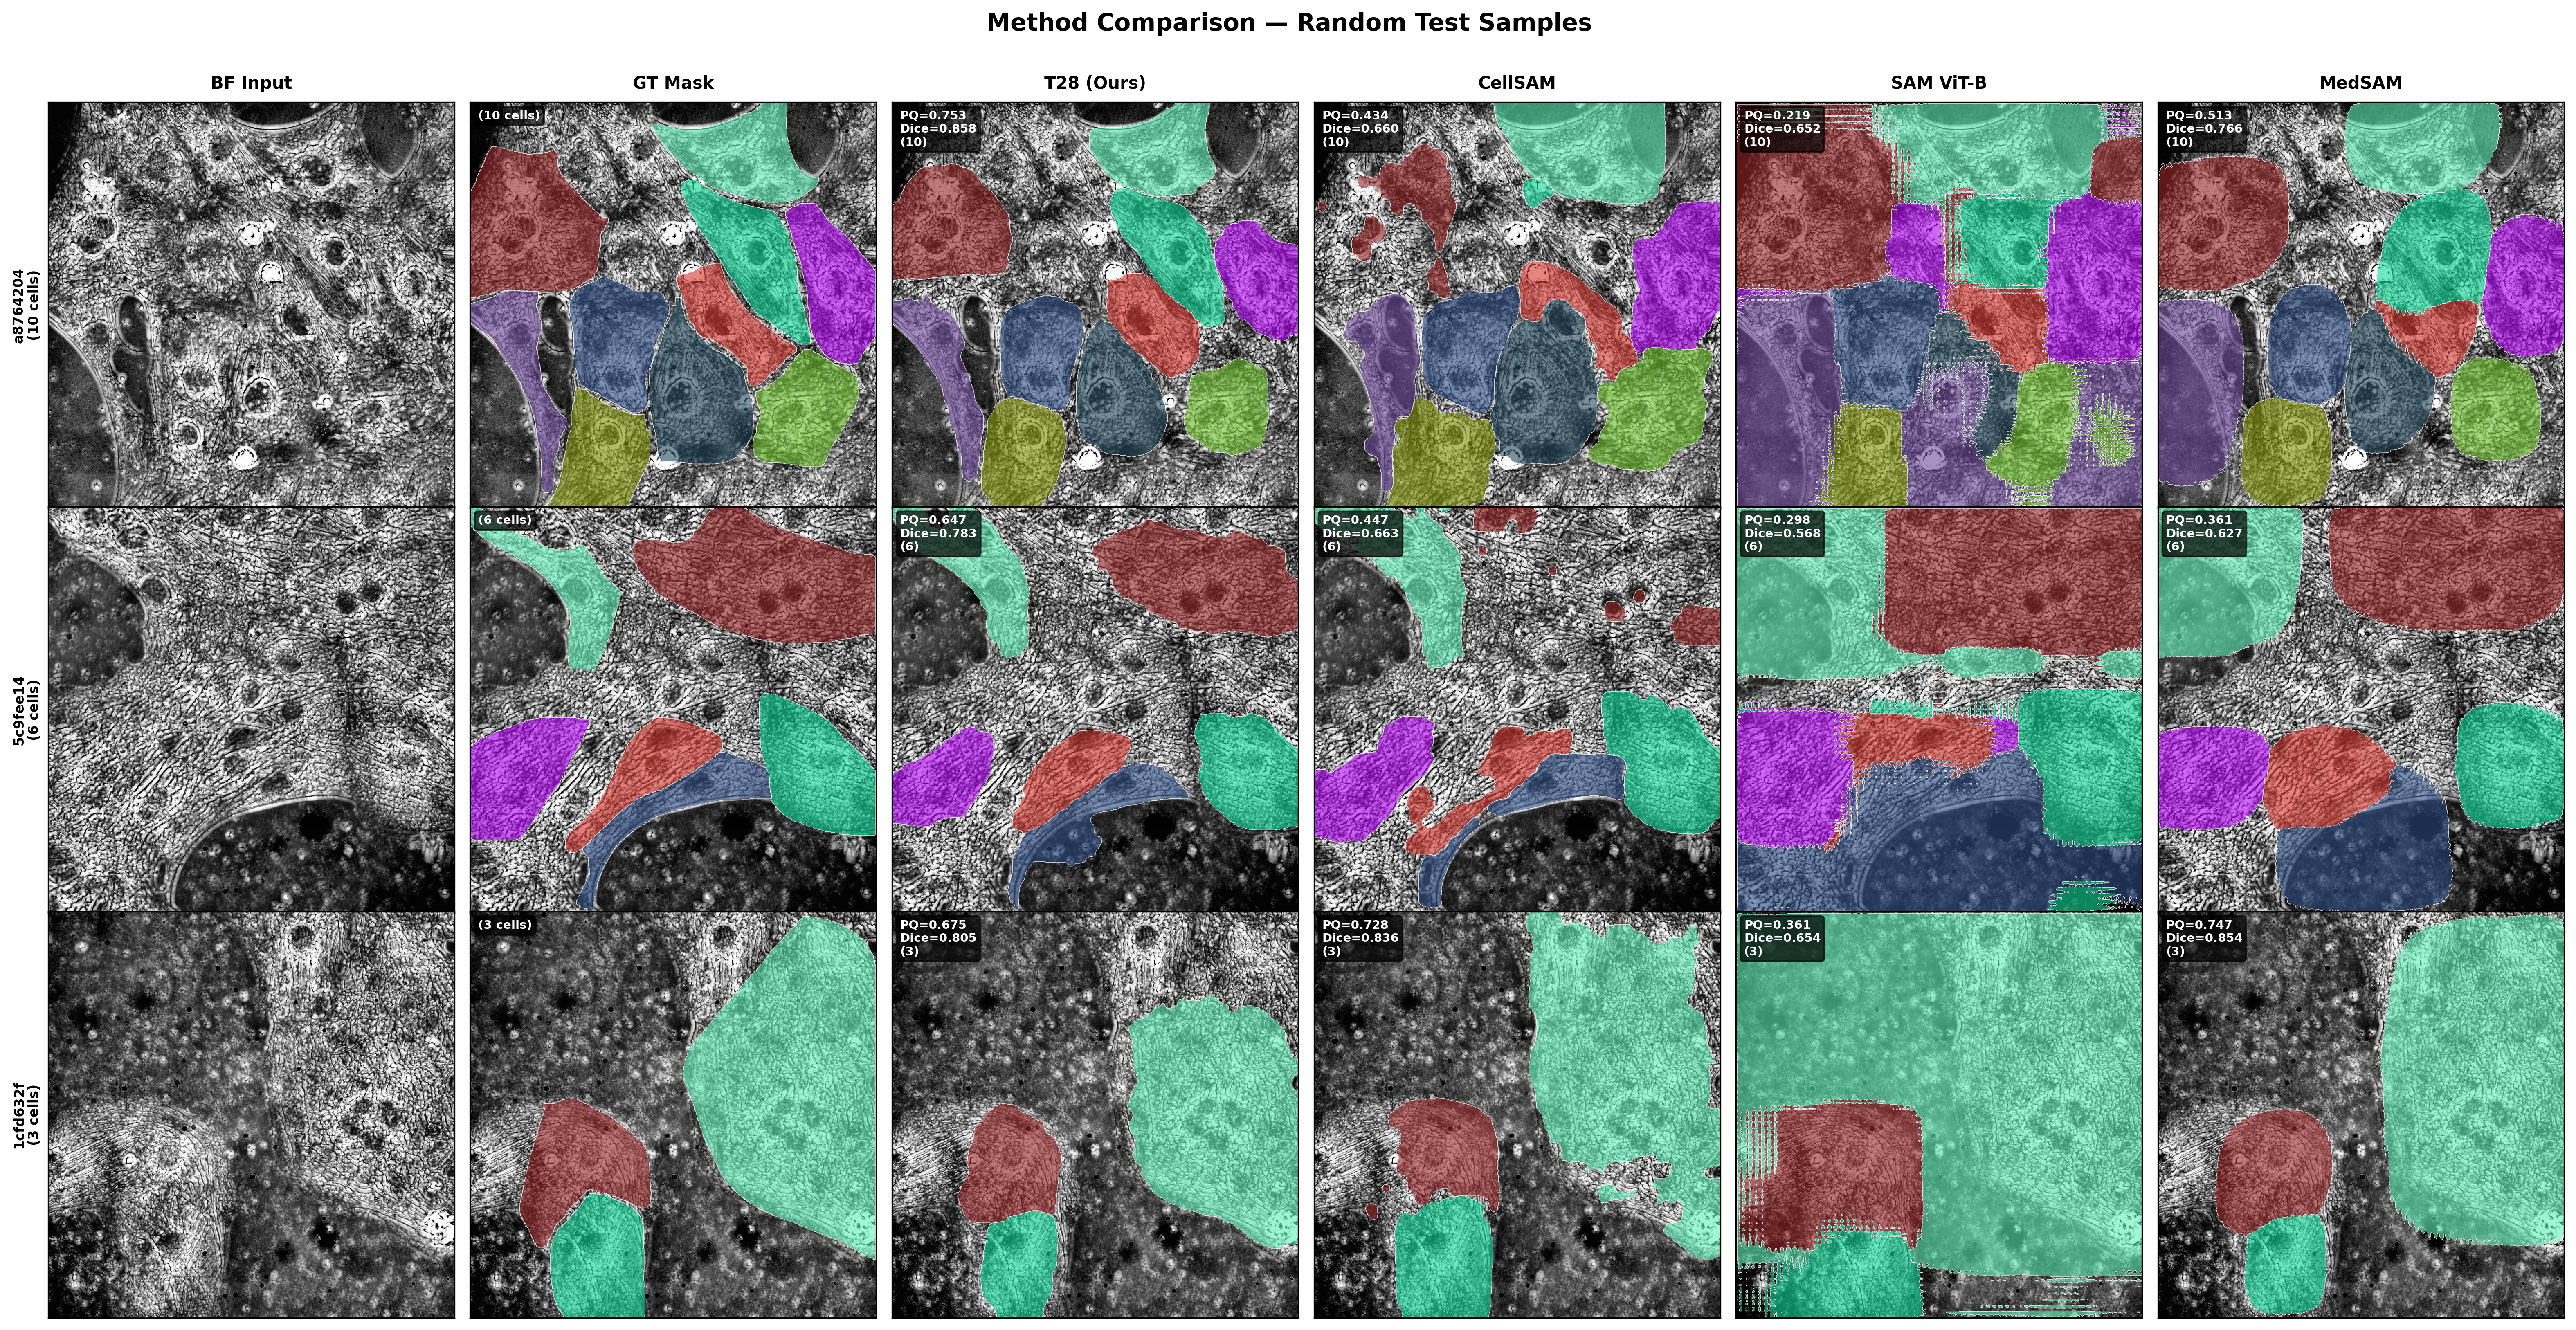
\includegraphics[width=\linewidth]{figures/paper_oracle_random3_no_cellpose_20260319.png}
  \caption{Oracle comparison on random test samples. With GT prompts, T28 yields high-quality masks, indicating that most end-to-end loss comes from detector prompt quality rather than mask refinement capacity.}
  \label{fig:t33g_t28_oracle_random3}
\end{figure}

\begin{figure}[t]
  \centering
  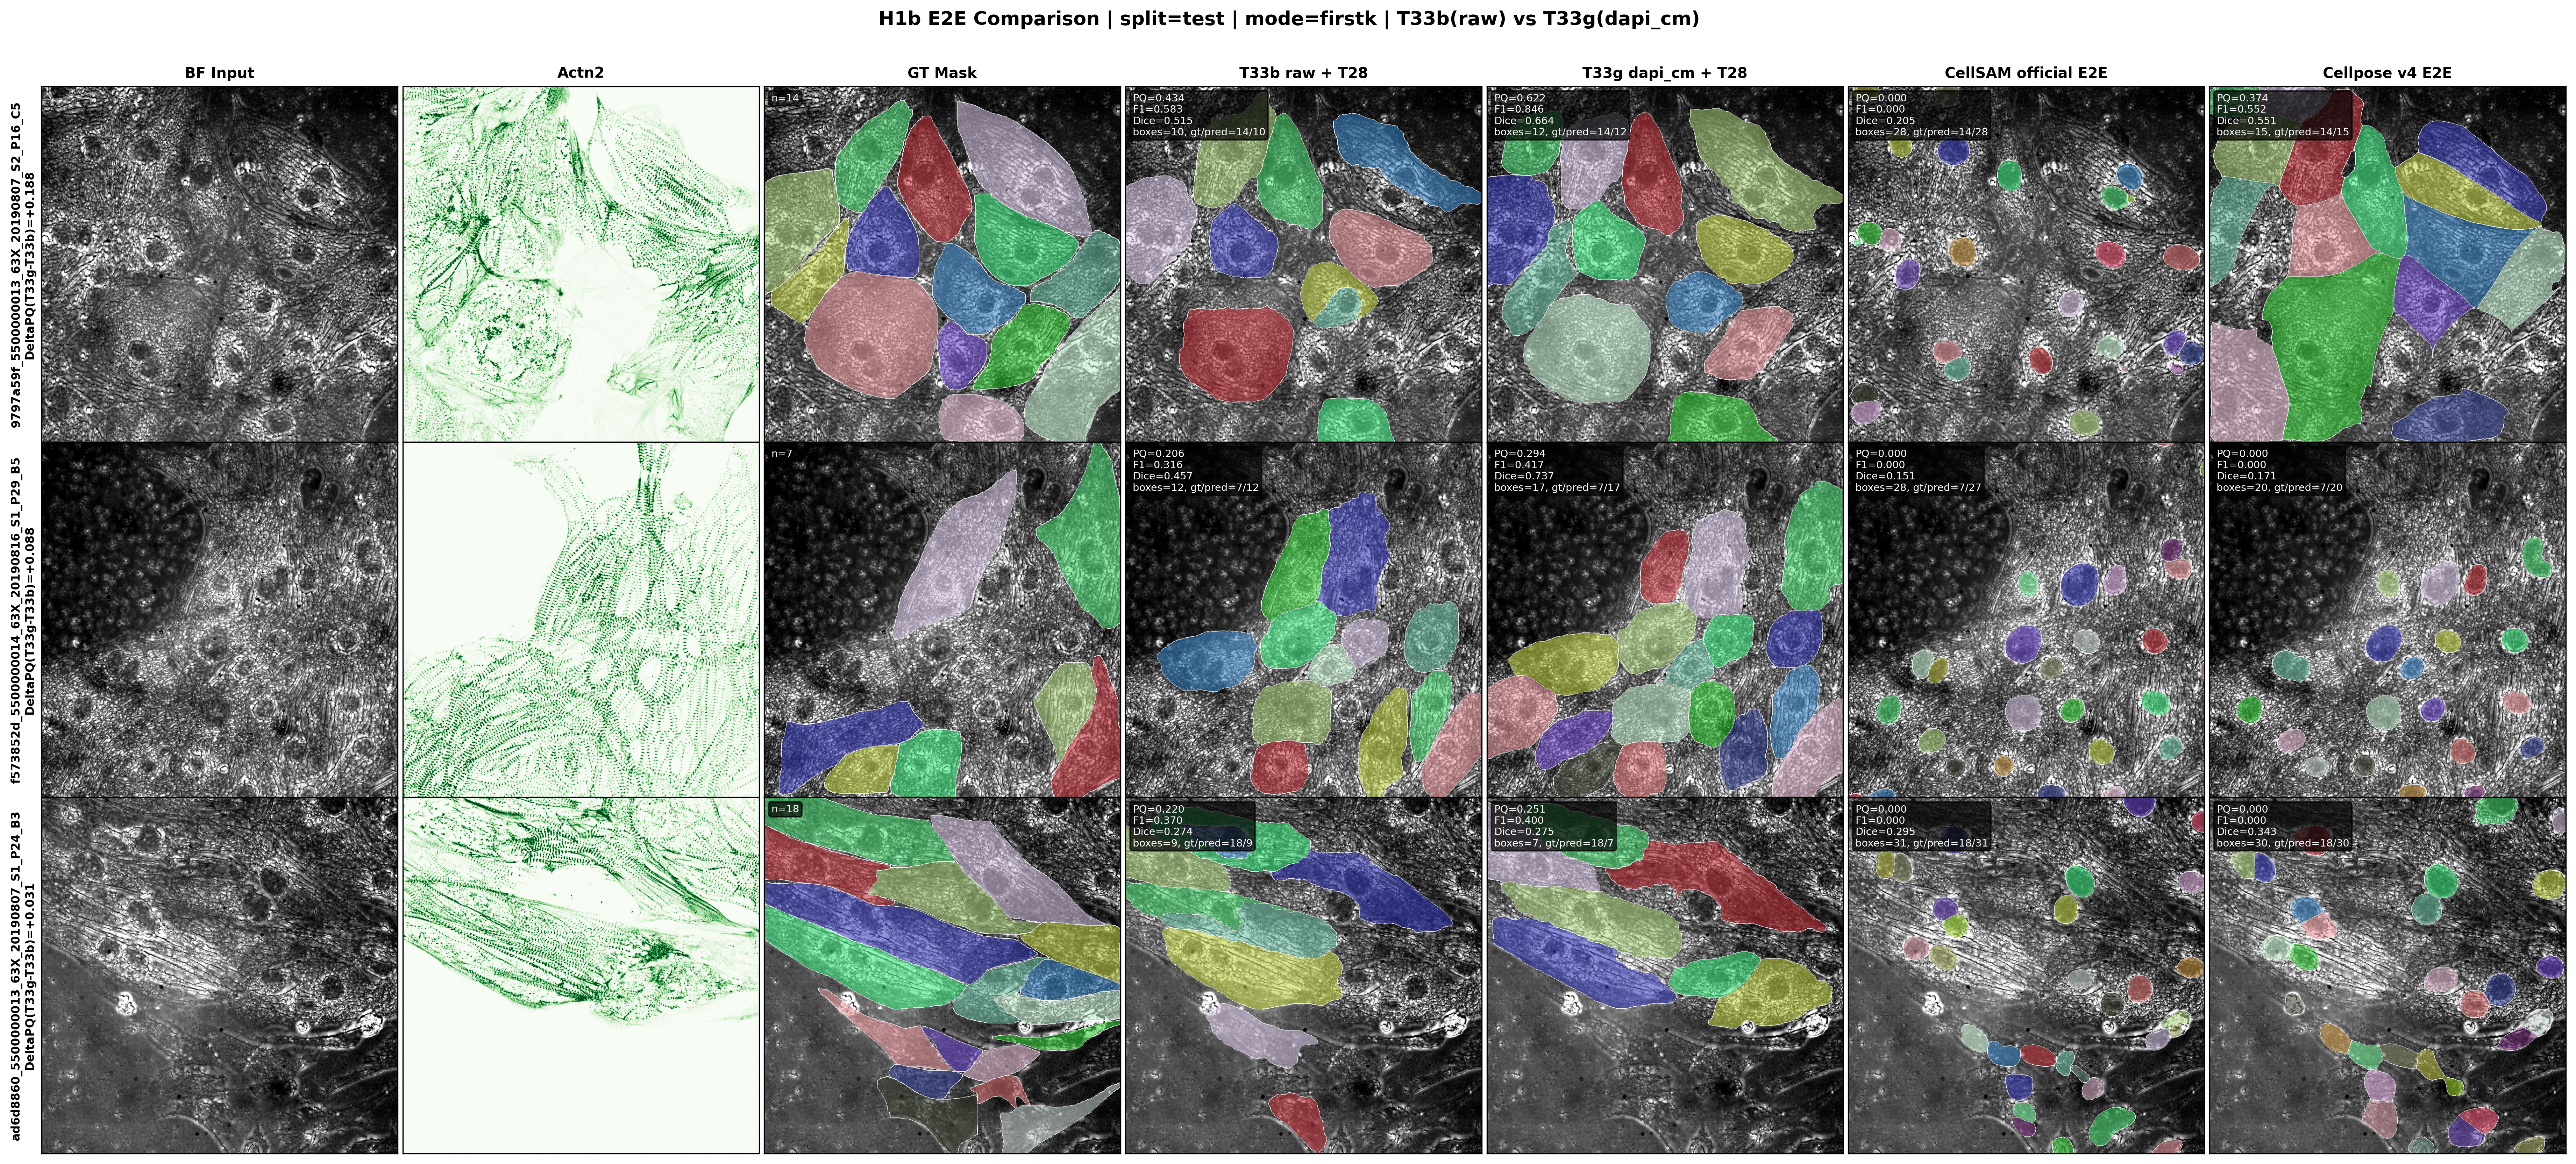
\includegraphics[width=\linewidth]{figures/t33g_t28_e2e_comparison_20260320.png}
  \caption{End-to-end qualitative comparison on three representative test samples. The T33g(dapi\_cm)+T28 route improves biologically plausible recovery over raw detector prompts while exposing known GT-v1 ambiguity cases.}
  \label{fig:t33g_t28_e2e_main}
\end{figure}

\begin{figure}[t]
  \centering
  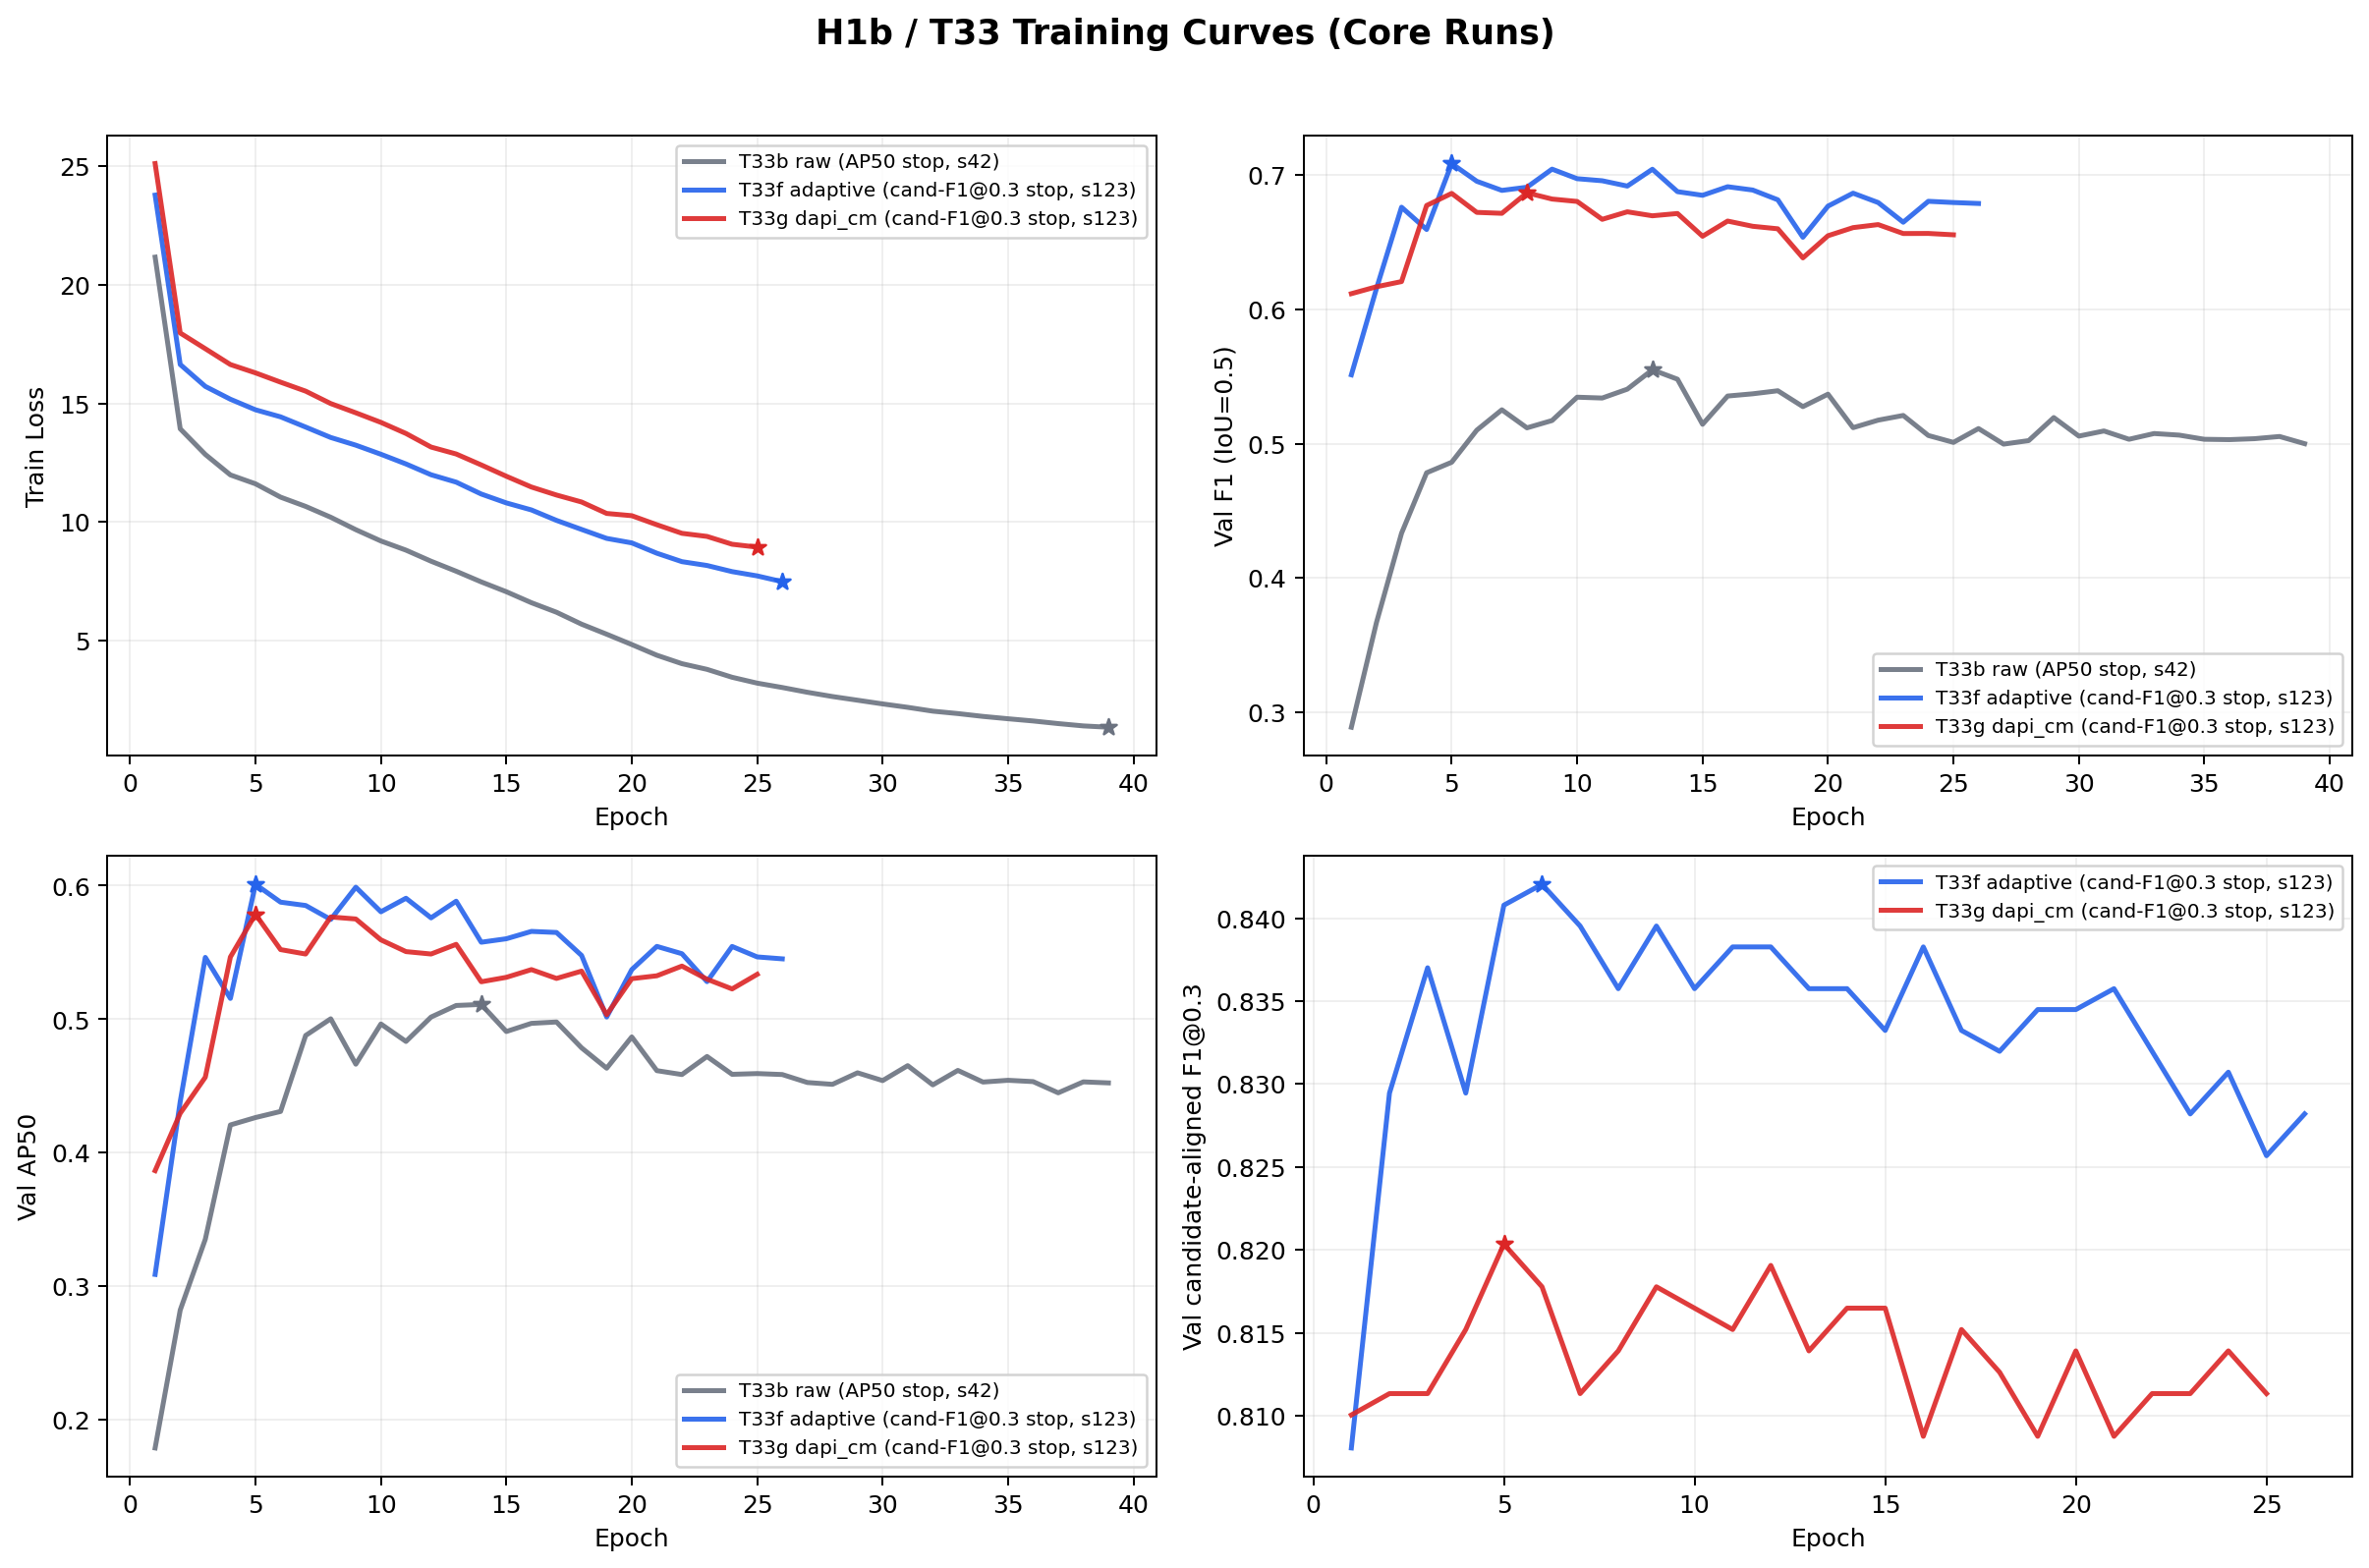
\includegraphics[width=\linewidth]{figures/t33_detector_training_curves_20260320.png}
  \caption{Training dynamics of T33 detector variants. Candidate-aligned F1@0.3 is the prior-aligned optimization target, while F1@0.5 and AP50 are auxiliary detector-quality monitors.}
  \label{fig:t33_detector_curves}
\end{figure}

GT-v1 contains likely missing or over-labeled instances in a small subset. This can suppress some end-to-end scores even when qualitative cardiomyocyte recovery is biologically plausible. Therefore, interpretation in Figure~\ref{fig:t33g_t28_e2e_main} is read jointly with metric evidence rather than as standalone proof.

\subsection{Prompt-Robustness Controls (Condensed Main-Text Anchor)}\label{prompt-robustness-controls-condensed-main-text-anchor}

To test whether simple mixed-prompt decoder retraining can close the Oracle-to-end-to-end gap, we ran three controls (\texttt{S2-E1/S2-E2/S2-E3}) initialized from the historical T27a route. The stable conclusion is negative: none of the controls improved end-to-end performance over the historical reference, and all reduced Oracle-side quality. Concretely, the best end-to-end control (\texttt{S2-E1}) still remains below the historical T27a reference by \texttt{0.024} PQ (\texttt{0.269} vs. \texttt{0.293}) and by \texttt{0.042} F1 (\texttt{0.455} vs. \texttt{0.497}), while also reducing Oracle PQ from \texttt{0.659} to \texttt{0.614}. This is an informative boundary result that supports the prompt-bottleneck diagnosis.

Therefore, the thesis does not promote mixed noisy-prompt decoder retraining as a main method branch. Detailed S2 settings and full metrics are reported in Appendix~B (\S\ref{s2-mixed-prompt-controls-supplementary-reference}).

\subsection{Provisional and Historical Observations}\label{provisional-and-historical-observations}

Not every useful experiment belongs in the main table. Some results are informative but should be written with weaker claims. Preliminary single-seed multi-channel observations are therefore kept in Appendix~B only, not promoted as body-level ablation evidence.

\subsubsection{T30 encoder adaptation is exploratory, not part of the current main result}\label{t30-encoder-adaptation-is-exploratory-not-part-of-the-current-main-result}

The T30 encoder-adaptation line (with historical T11 context) provided a modest positive signal. The best historical encoder-adaptation result reached \texttt{PQ\ =\ 0.494}, which is higher than Best Config but still below the current locked T27a \texttt{test73} reference. This keeps encoder adaptation as a future-work direction rather than a central thesis claim at the current stage.

\subsubsection{Neighbor/overlap exclusion losses are a negative result}\label{neighboroverlap-exclusion-losses-are-a-negative-result}

The P2-A experiments consistently degraded performance. The best delayed-activation setting still peaked before the extra losses became active, which indicates that naive repulsion-style losses conflict with the core segmentation objective on dense cardiomyocyte scenes.

This is worth keeping in the thesis because it shows that not all intuitively appealing structural losses are beneficial in practice.
